\documentclass[authoryear,11pt]{elsarticle}

%This eliminates the `Preprint submitted to...' footer on the first page
\makeatletter
\def\ps@pprintTitle{%
 \let\@oddhead\@empty
 \let\@evenhead\@empty
 \def\@oddfoot{}%
 \let\@evenfoot\@oddfoot}
\makeatother

\usepackage{amssymb}
\usepackage{amsthm}
\usepackage{caption}
\usepackage{amsmath}
\usepackage{morefloats}
\usepackage{bbm}        %To allow \mathbb{1}

\usepackage{rotating}   %To turn tables sidewaystable
\usepackage{graphicx}
\usepackage{setspace}
\usepackage{hyperref}

%\onehalfspacing

%\setlength{\parindent}{0pt}

\usepackage[top=3.5cm,bottom=3.75cm,left=2.45cm,right=2.45cm]{geometry}% by courtesy of Mico

\begin{document}
\begin{frontmatter}
\title{MFE Economics\\Problem set 3}
\end{frontmatter}

%%%%%%%%%%%%%%%%%%%%%%%%%%%%%%%%%%%%%%%%%%%%%%%%%%%%%%%%%%%%%%%%%%%%%%%%%%%%%%%%%%%%%%%%%%%%%%%%%%%%%%%%%%%%%%%%%%%%%%%%%%%%%%%%%%%%%%%%%%%%%%%%%%%%%%%%
%%%%%%%%%%%%%%%%%%%%%%%%%%%%%%%%%%%%%%%%%%%%%%%%%%%%%%%%%%%%%%%%%%%%%%%%%%%%%%%%%%%%%%%%%%%%%%%%%%%%%%%%%%%%%%%%%%%%%%%%%%%%%%%%%%%%%%%%%%%%%%%%%%%%%%%%

\section{Stochastic growth model}

\begin{itemize}
\item Technology process
\begin{gather*}
Y_{t}=K_{t}^{\alpha }\left( \theta _{t}L_{t}\right) ^{1-\alpha } \\
\theta _{t}=e^{z_{t}}>0 \\
z_{t}=\mu (1-\rho )t+\rho z_{t-1}+\varepsilon _{t}
\end{gather*}
\item Technology has trend component and persistent shocks
\begin{equation*}
\log \theta _{t}=\mu (1-\rho )t+\rho \log \theta _{t-1}+\varepsilon _{t}
\end{equation*}
\item	Firm maximises profits
\begin{equation*}
\underset{K_{t},L_{t}}{\max }\left( K_{t}^{\alpha }\left(\theta_{t}L_{t}\right) ^{1-\alpha }-w_{t}L_{t}-r_{t}K_{t}\right)
\end{equation*}
\item	Representative household maximizes lifetime utility
\begin{eqnarray*}
\underset{L_{t+s},C_{t+s}, K_{t+s}}{\max } &E_{t}& \sum\limits_{s=0}^{\infty} \beta^{s} (\log{C_{t+s}} - \chi L_{t+s}) \\
s.t.&& \\
K_{t+s+1} = r_{t+s} K_{t+s} + w_{t+s} L_{t+s} - C_{t+s} \; \forall s\geq 0 &&\\
K_{t} \; given&& \\
 \lim_{T\rightarrow \infty} E_{t} [\Lambda_{t,T} K_{t+1} ] \geq 0&&
\end{eqnarray*}
\end{itemize}

\begin{itemize}
\item	Derive the firm and household optimality conditions.\footnote{Note this is very similar to the model discussed in lecture 2 but with an expectation operator $E_{t}$ floating around, which doesn't hugely change the appearance of the expressions - the main difference is allowing for non-trivial labor supply decisions.}
\item	Show that the only stable solution has (like in the lecture 2 model) implies $\frac{Y_{t}}{C_{t}} = \frac{1}{1-\alpha \beta}$
\item	Using the fact that (as you should have shown in the first part of the question) firm optimality implies the real wage is equal to the marginal product of labor, show that $\frac{Y_{t}}{C_{t}} = \frac{1}{1-\alpha \beta}$, combined with the household's labor-consumption optimality condition, yields an expression for equilibrium $L_{t}$ in terms of deep parameters ($\alpha, \beta, \chi$)
\item	Does equilibrium labor vary over time?
\item	Payments to capital (or capitalists that own them) are $r K_{t}$. Show that the capital share of income ($\frac{r_{t} K_{t}}{Y_{t}}$) equals $\alpha$ - so the labor share is $1-\alpha$. What number should we set $\alpha$ to be for the US, on this basis? Consult \href{https://www.bls.gov/opub/mlr/2017/article/estimating-the-us-labor-share.htm}{here} and \href{https://fred.stlouisfed.org/series/PRS85006173}{here}. Briefly discuss/critique your answer.
\item	Given the previous answers and assuming $\beta = 0.95$, what should $\chi$ be for steady state $L$ to be $1/3$ of the time endowment ($8$ hours out of a $24$ hour day spent working)
\end{itemize}


\subsection*{Answers}

\begin{itemize}
	\item \emph{Firm's optimality conditions.} Every period, firm faces a simple static problem of choosing capital and labour to maximize its profit, taking factor prices $w_t$ and $r_t$ as given:
	\[
		\max_{K_t,L_t} \ K_t^\alpha (\theta_tL_t)^{1-\alpha} - w_tL_t - r_tK_t
	\]
	First order conditions (FOCs) with respect to $K_t$ and $L_t$, respectively, are:
	\[
		r_t = \underbrace{\alpha K_t^{\alpha-1}(\theta_tL_t)^{1-\alpha}}_{\text{Marginal product of capital}}
	\]
	\[
		w_t = \underbrace{(1-\alpha) K_t^{\alpha}\theta_t^{1-\alpha}L_t^{-\alpha}}_{\text{Marginal product of labour}}
	\]
	Using $Y_t = K_t^\alpha(\theta_tL_t)^{1-\alpha}$, the above conditions could be simplified:\footnote{If you do not see this, multiply and divide the right hand side of the first FOC by $K_t$, and the right hand side of the second FOC by $L_t$}
	\begin{gather}
		r_t= \alpha \frac{Y_t}{K_t}
		\label{eq:firm_foc_k}
	\end{gather}
	\begin{gather}
		w_t = (1-\alpha) \frac{Y_t}{L_t}
		\label{eq:firm_foc_l}
	\end{gather}
	
	\emph{Household's optimality conditions.} Substitute the budget constraint in to get an unconstrained maximization problem:
	\[
		\max_{\{L_{t+s},K_{t+s+1}\}_{s=0}^\infty} \ \mathbb{E}_t \ \sum_{s=0}^{\infty} \beta^s \ln \underbrace{\left(r_{t+s} K_{t+s} + w_{t+s} L_{t+s} - K_{t+s+1}\right) }_{C_{t+s}}- \chi L_{t+s}
	\]
	First order condition with respect to $L_t$ is:\footnote{Hint: to take this first order condition at $t$, you only need to consider part of the problem when $s=0$.}
	\begin{gather}
		\chi = \frac{w_t}{C_t}
		\label{eq:hh_foc_l}
	\end{gather}
	This is the \textbf{intratemporal} optimality condition. On the left hand side we have marginal disutility of working, while on the right hand side we have marginal utility from working a little bit more and consuming extra earnings. The rational household equalises marginal cost with marginal benefit.
	
	First order condition with respect to $K_{t+1}$ is:\footnote{Hint: to take this first order condition at $t$, you need to consider part of the problem when $s=0$, but also when $s=1$, since current savings will be repayed at $t+1$ with interest.}
	\begin{gather}
		\frac{1}{C_{t+1}} = \beta \ \mathbb{E}_t \frac{1}{C_{t+1}} r_{t+1}.
		\label{eq:euler}
	\end{gather}
	This is the \textbf{(intertemporal) Euler equation}. On the left hand side we have marginal disutility of saving at $t$\footnote{which would be the marginal utility of consuming extra unit of resources in period $t$ instead.}, whereas on the right hand side we have the discounted expected marginal utility of saving (given the ``transformation technology'' $r_{t+1}$).
	
	\item In the equilibrium, the market for capital clears in every period: interest rate adjusts such that households' savings equal firms' demand for capital. Rational households understand how the interest rate will be determined in the future. We can thus substitute firms' optimality condition \eqref{eq:firm_foc_k} at $t+1$ into the Euler equation \eqref{eq:euler} to get:
	\[
		\frac{1}{C_{t+1}} = \beta \ \mathbb{E}_t\alpha\frac{Y_{t+1}}{C_{t+1}K_{t+1}},
	\]
	or, recognizing that $K_{t+1}$ is predetermined at $t+1$:
	\[
		\mathbb{E}_t \frac{Y_{t+1}}{C_{t+1}} = \frac{1}{\alpha\beta}\frac{K_{t+1}}{C_t} .
	\]
	The output in every period can be either saved or consumed: $Y_t=K_{t+1}+C_t$ (market clearing for final good). Substituting $K_{t+1}$ into the equation above, we get a first order difference equation in $\left(\frac{Y_t}{C_t}\right)$:
	\[
		\mathbb{E}_t \left(\frac{Y_{t+1}}{C_{t+1}}\right) = \frac{1}{\alpha\beta}\left(\frac{Y_{t}}{C_t}\right)  - \frac{1}{\alpha\beta}
	\]
	\begin{figure}[!htb]
		\center{\includegraphics[width=0.6\textwidth]{phase_diag}}
		\caption{\label{fig:phase_diag} Phase diagram for $\mathbb{E}_t \frac{Y_{t+1}}{C_{t+1}} = \frac{1}{\alpha\beta}\frac{Y_{t}}{C_t}  - \frac{1}{\alpha\beta}$}
	\end{figure}
	Figure \ref{fig:phase_diag} illustrates the phase diagram for this equation. If we start at $\left(\frac{Y_{t}}{C_t}\right)$ above $\left(\frac{Y}{C}\right)^*$, the ratio of output to consumption will diverge to $+\infty$ in expectation, clearly violating the \textbf{transversality condition}: rational player does not leave unconsumed resources on the table. If we start below $\left(\frac{Y}{C}\right)^*$, $\left(\frac{Y_{t}}{C_t}\right)$ will diverge to $-\infty$, clearly violating the feasibility requirement (\textbf{No-Ponzi constraint}): player cannot finance consumption by forever increasing debt. Therefore, the only stable solution is when $\left(\frac{Y_{t}}{C_t}\right)$ is constant and equal $\left(\frac{Y}{C}\right)^*$ in every period. We can find it by solving:
	\[
		\left(\frac{Y}{C}\right)^* = \frac{1}{\alpha\beta}\left(\frac{Y}{C}\right)^*  - \frac{1}{\alpha\beta},
	\]
	which yields
	\begin{gather}
		\left(\frac{Y}{C}\right)^* = \frac{1}{1-\alpha \beta}.
		\label{eq:y_to_c}
	\end{gather}
	
	\item In the competitive equilibrium, the real wage level equalises the households' labour supply and firms' labour demand. Plug the firms' FOC \eqref{eq:firm_foc_l} into the households' optimality condition \eqref{eq:hh_foc_l}:
	\[
		\chi = \frac{1-\alpha}{L_t} \frac{Y_t}{C_t} = \frac{1-\alpha}{(1-\alpha\beta)L_t},
	\]
	where the second equality is obtained by using \eqref{eq:y_to_c}. Now express $L_t$ to get:
	\begin{gather}
		L_t = \frac{1-\alpha}{\chi(1-\alpha\beta)}
		\label{eq:eq_labour}
	\end{gather}
	
	\item We can see that equilibrium employment is constant in this simple model with linear disutility of working.
	
	\item Using \eqref{eq:firm_foc_k} we can write the capital's share of income as:
	\[
		\frac{rK_t}{Y_t} = \frac{\alpha \frac{Y_t}{K_t}K_t}{Y_t} = \alpha,
	\]
	which simply is the capital's share in the constant return to scale Cobb-Douglas production function. It follows that the share of income that goes to labour in this model is $1-\alpha$. 
		
	Historically, labour share of income was around $\frac{2}{3}$, so we can set $\alpha=\frac{1}{3}$. 
	
	Note, however, that labour share seems to be going down in the last 20 years or so. Can it be the ``new normal'': AI, automation, etc? 
	
	\item Using \eqref{eq:eq_labour}, we can set $L_t=\frac{1}{3}$, and immediately solve for the required coefficient $\chi$:
	\[
		\frac{1}{3} = \frac{1-\frac{1}{3}}{\chi\left(1-\frac{1}{3}\cdot 0.95\right)},
	\]
	which yields $\chi \approx 3$. This is a gentle intro to how we \textbf{calibrate} structural macroeconomic models.

\end{itemize}


\section{Correcting an inefficiency with a Pigouvian subsidy}
Consider the monopolistically competitive firm discussed in the previous problem set. The chosen output level (reflecting the chosen price) is such that price is a markup on marginal cost. This is inefficient. Effectively, the price reflects the marginal valuation of the output by the marginal consumer. Since the price is above marginal cost it means that at $Y^{\ast}$ (the output level implied by the chosen price, $P^{\ast}$, given the demand curve) the `consumer' values an extra marginal unit more than the cost to the firm of producing that marginal unit (the marginal cost), thus there are possible gains from trade that are not being exploited - the consumer would be willing to pay a price between $MC(Y^{\ast})$ and $P(Y^{\ast})$ for that good. The firm would be fine with that and so would the consumer - implying a Pareto improvement. This will be possible right up to the point, call it $Y^{Eff}$, where we have price = marginal cost.

For efficiency we would like to somehow induce the firm to produces $Y^{Eff}>Y^{\ast}$. Note that the firm produces to the point at which marginal cost = marginal revenue where the latter lies below the demand curve. One can offer a subsidy to the firm to change the `private' marginal cost it faces. In particular, if the `government' offers to pay fraction $\tau$ of the wage then for a given wage received by a worker, $W_{t}$, the firm only pays $(1-\tau)W_{t}$ - so from the firm's perspective this lowers their marginal cost. Call this private marginal cost $\widehat{MC}(Y_{t}) = \frac{(1-\tau)W_{t}}{MPN_{t}} = (1-\tau)MC(Y_{t})$ (recall marginal cost is wage paid by firm divided by the marginal product of labor, at the firm's privately optimal choice).

What value should $\tau$ \href{https://en.wikipedia.org/wiki/Pigovian_tax}{(a `Pigouvian' tax)} take to induce the firm to produce $Y^{Eff}$? HINT: The firm will still produce to the point where its \emph{private} MC = MR

\subsection*{Answers}
Since we want output to be produced to the point where $P_{t} = MC_{t}$ i.e. price equals the `true' marginal cost and the firm will set $P_{t} = \mathcal{M}\widehat{MC}_{t}$ we require $1-\tau = \mathcal{M}^{-1}$. Recalling the definition of $\mathcal{M}$, this implies $\tau = \varepsilon^{-1}$. Going back to diagramatic analysis, figure \ref{fig:monop_comp_subsidy} illustrates the impact of confronting the firm with a lower effective marginal cost curve that induces it to produce $Y^{Eff}$. Given the appropriate choice of $\tau$ the firm sees its private marginal cost as equaling marginal revenue at a higher output level than before. At that output level the `true' marginal cost is equal to price (and thus the marginal valuation of the consumer) and we have exhausted all gains from trade - we have a Pareto efficient situation (in the narrow partial equilibrium sense considered in this question).

As a final point note that by eliminating the deadweight loss (the Harberger triangle vanishes when $P=MC$) we have `increased the size of the pie'. We have generated additional production that can be allocated so as to make everyone (firm and household) weakly better off and some agents strictly better off. In this case we achieved it by subsidizing the firm. Because the pie is bigger the government is able to fund this subsidy, which is often called a `Pigouvian' susbidy after the eminent economist \href{https://en.wikipedia.org/wiki/Arthur_Cecil_Pigou}{A. C. Pigou}, who studied corrective taxes and subsidies to deal with market failures deriving from misaligned tradefoffs/implicit prices.

\begin{figure}[!htb]
\center{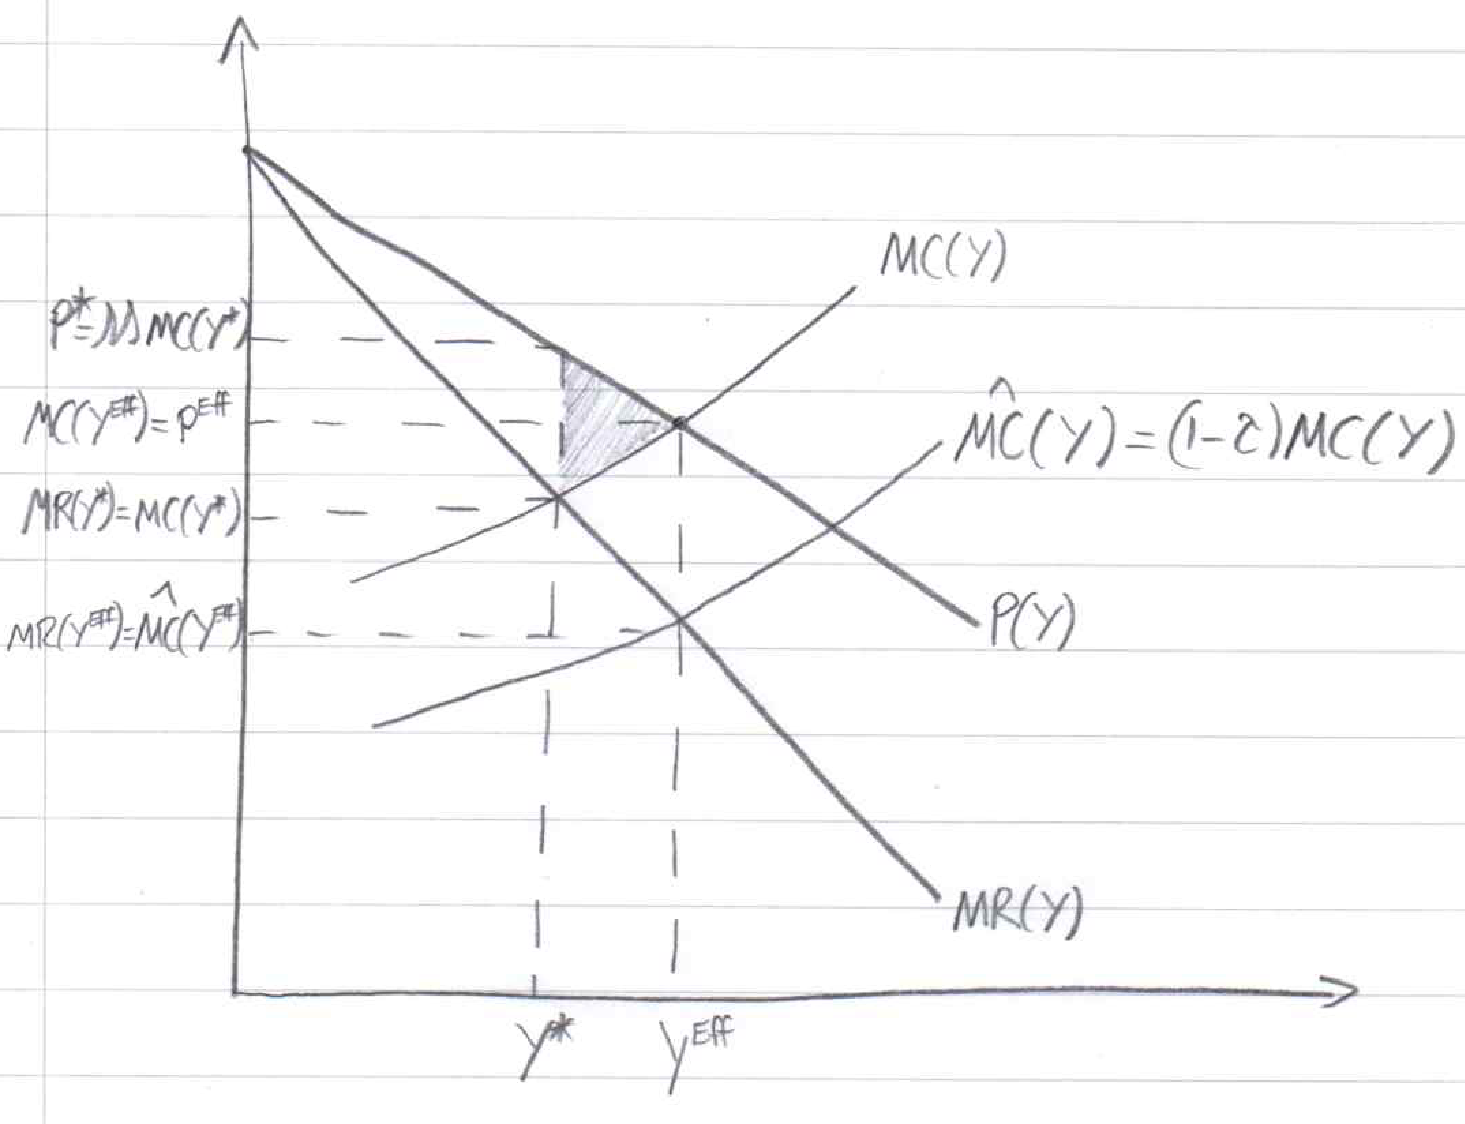
\includegraphics[width=0.6\textwidth]{monop_comp_subsidy_graph.pdf}}
\caption{\label{fig:monop_comp_subsidy} Price setting by a firm facing a downward sloping demand curve and a subsidized wage set to induce an efficient level of output}
\end{figure}

\section{Optional: Calvo Pricing}
\textbf{RB: See the Gali textbook for discussions of Calvo pricing. This question is to get you to do a bit of thinking about this pricing protocol before I cover it in class. If you find it tricky, don't worry, as I will be going over it.}

Under the \href{https://www.sciencedirect.com/science/article/pii/0304393283900600}{Calvo (1983)} pricing protocol a firm faces a probability, $\theta$, of being unable to reset its price in any given period and this probability is independent of how long any given price has so far been prevailing. Sometimes people imagine a `Calvo fairy' who, in any given period, will wave a wand over the firm's head (with probability $1-\theta$) and allow them to reset their price.
\begin{itemize}
\item	What is the probability of a price prevailing $j$ periods after it has been chosen? \textit{HINT: Think about the sequence of fairy arrivals or non arrivals and remember the probabilities are independent over time so you can multiply appropriate probabilities together\ldots}
\item	Show that the expected duration of a price (i.e. how many periods on average will it prevail before being reset) is $(1-\theta)^{-1}$? Note: Don't spend more than $20$ mins on this bit - either it will pop into your head how to rearrange the algebra, or it won't - but try for $20$mins\ldots
\item	What value of $\theta$ would I pick my for my (quarterly) model to match real world data that suggests prices typically prevail for $3$ quarters?
\end{itemize}

\subsection*{Answers}
The probability that a price lasts for only one period is $1-\theta$ - that is, the probability that in the first period after setting the price, the firm gets to set it again. The probability that the price lasts for two periods is the probability that it is fixed for one period multiplied by the probability that it will be reset in the following period, conditional on it having not been reset after one period. But since the Calvo probability is \emph{independent of how long a price has been prevailing}, this latter probability is always simply $1-\theta$. This logic then extends\ldots
\begin{itemize}
\item	Pr[Prevails for 1 period] 	= $1-\theta$
\item	Pr[Prevails for 2 periods]	= Pr[No reset through second period] $\times(1-\theta)$ = $\theta(1-\theta)$
\item	Pr[Prevails for 3 periods]	= Pr[No reset through third period] $\times(1-\theta)$ = $\theta^{2}(1-\theta)$
\item	etc
\item	Pr[Prevails for j periods]	= Pr[No reset through $j^{th}$ period] $\times(1-\theta)$ = $\theta^{j-1}(1-\theta)$
\end{itemize}
Thus, the probability is $\theta^{j-1}(1-\theta)$

As to the expected duration of the price, we note that the duration is a random variable. We have just found the probability associated with each of its possible values so to find the expected duration we simply calculate the mean, which is a probability-weighted average:
\begin{eqnarray*}
E[Duration] 	&=& \sum\limits_{j=1}^{\infty} Pr[\text{Prevails for j periods}] j \\
			&=& \sum\limits_{j=1}^{\infty} (1-\theta) \theta^{j-1} j	\\
			&=& (1-\theta)  \sum\limits_{j=1}^{\infty} \theta^{j-1} j
\end{eqnarray*}
Thus, we need to figure out the value of $\sum\limits_{j=1}^{\infty} \theta^{j-1} j$. If we write it out `carefully' we see that it has a clean structure\ldots
\begin{eqnarray*}
\sum\limits_{j=1}^{\infty} \theta^{j-1} j	&=& 1 + 2\theta + 3 \theta^2 + 4\theta^3 +\ldots	\\
										&=& 1 + \theta + \theta^2 + \theta^3 + \ldots	\\
										& &  + \theta + \theta^2 + \theta^3 + \ldots	\\
										&&   + \theta^2 + \theta^3 + \ldots	\\
										&&	 + \ldots
\end{eqnarray*}
but this can be re-written as follows
\begin{eqnarray*}
\sum\limits_{j=1}^{\infty} \theta^{j-1} j	&=& 1 + \theta + \theta^2 + \theta^3 + \ldots	\\
										& &  + \theta(1 + \theta + \theta^2 + \theta^3 + \ldots) \\
										& &  + \theta^2(1 + \theta + \theta^2 + \theta^3 + \ldots) \\	
										&&   + \ldots
\end{eqnarray*}
which, in turn, can be re-written as
\begin{eqnarray*}
\sum\limits_{j=1}^{\infty} \theta^{j-1} j	&=& \sum\limits_{k=0}^{\infty}\theta^{k} \left(  \sum\limits_{j=0}^{\infty}\theta^{j} \right)	\\
										&=& \frac{1}{1-\theta} \sum\limits_{j=0}^{\infty}\theta^{j}				\\
										&=& \frac{1}{1-\theta} \frac{1}{1-\theta}
\end{eqnarray*}
Thus we have that 
\[
E[Duration]  = (1-\theta) \sum\limits_{j=1}^{\infty} \theta^{j-1} j =  \frac{1}{1-\theta}
\]
Thus, as one would expect, the higher the degree of price stickiness (the higher the probability, $\theta$, of not being able to adjust) the longer is the expected duration of a price. Now, if one has data on prices from the real world, then one can get a sense of what $\theta$ should be by calculating the average duration in the data and setting $\theta$ to match it. Of course, this model is too simple to capture the many other properties of the distribution of price duration, but it is a useful simplification.\footnote{Once $\theta$ is pinned down by matching the mean duration, we have no other degrees of freedom to match the variance, skew or whatever other moments of the price duration distribution observed in the real world.}

If we want to pick $\theta$ to match the given real world `moment' we require $(1-\theta)^{-1} = 3$. This implies that, after rearranging, $\theta = \frac{2}{3}$.


\section{Autoregressive processes}
In the models we consider, there are random `shock' or `driving' processes that are exogenous to the model.\footnote{You can brush up on random variables \href{https://en.wikipedia.org/wiki/Random_variable}{here}, on Normal variables \href{https://en.wikipedia.org/wiki/Normal_distribution}{here} and on expected value (or `the mean') \href{https://en.wikipedia.org/wiki/Expected_value}{here}.} In our case these shocks (technology, time preference and monetary policy) will constitute the `state' of the economy in the sense that all the endogenous variables (consumption, output, wages, interest rates) will in equilibrium be expressible as functions of these three variables (or subsets thereof, depending on the model). All the shocks we consider, when logged, follow an autoregressive process of order $1$ or, for short, an $AR(1)$. Consider the technology shock $A_{t}$ from the production function $Y_{t} = A_{t}N_{t}^{1-\alpha}$. When expressed in logs it follows this process\footnote{Note that is convenient to model it this way as it means that $A_{t}$, while random, will always be positive (as makes sense for a technology term that multiplies - some function of - labor to produce non-negative output). Frequently in economics or finance we use the exponential of a random variable to obtain a transformed random variable that is positive. In fact, exponentials have other nice properties when working with Normal distributions.}
\begin{eqnarray}
a_{t} 			&=& \rho_{a} a_{t-1} + \varepsilon_{a,t} 	\label{eqn:ar1} \\
\varepsilon_{a,t} &\overset{iid}{\sim}& N(0,\sigma^{2}_{a})	\nonumber \\
a_{t}			&\equiv& \log{(A_{t})} \nonumber
\end{eqnarray}

The random variable, $\varepsilon_{a,t}$  (what I will often refer to as an `innovation'), is a Gaussian or `Normal' variable with zero mean ($E_{t}[\varepsilon_{a,t+1}] = 0$) and variance, $\sigma^{2}_{a}$ ($E_{t}[(\varepsilon_{a,t+1} - 0)^{2}] = \sigma^{2}_{a}$). It is also independently and identically distributed (iid) which means that there is no dependence between its draws in different periods or between its draw and any other variables and the distribution from which it is drawn ($N(0,\sigma^{2}_{a})$) is constant over time. The parameter $\rho_{a}$ will be referred to as a `persistence' parameter. We will always (in this course) consider cases where $|\rho_{a}| \in (0,1)$ - in the language of stochastic processes, this ensures that it is a `stationary' process.

\begin{itemize}
\item	Show that\footnote{HINT: Use equation (\ref{eqn:ar1}) but for earlier periods ($a_{t-1}$, $a_{t-2}$ etc.) to repeatedly replace the lagged values of $a_{t}$ on the right hand side of equation (\ref{eqn:ar1}).}
\begin{equation}
a_{t} = \sum\limits_{j=0}^{J-1} \rho_{a}^{j} \varepsilon_{a,t-j} + \rho_{a}^{J} a_{t-J} \label{eqn:sum_ar}
\end{equation}
\end{itemize}

Suppose data started in $t=0$, so that $a_{0}$ is just given to us, then we just set $J=t$ in the above expression. If there is no explicit starting point then we can use the assumption on $|\rho_{a}| \in (0,1)$ to state
\[
a_{t} = \sum\limits_{j=0}^{\infty} \rho_{a}^{j} \varepsilon_{a,t-j}
\]
since $\rho_{a}^{J} a_{t-J} \to 0$ as $J \to \infty$. Intuitively, if the effects of shocks dies of to zero in the limit - and given that our shocks are well behaved - we can ignore the last term in expression (\ref{eqn:sum_ar}) you just derived because it gets arbitrarily small.

\begin{itemize}
\item	What is the effect of an innovation $j$ periods ago on $a_{t}$ (i.e. the effect of $\varepsilon_{a,t-j}$)?
\item	What is the effect of an innovation in $t$ on $a_{t+1}$? On $a_{t+2}$? On $a_{t+j}$?
\end{itemize}

Any effect an innovation in $t$ has on future values of $a_{t}$, say $a_{t+j}$,  may be flooded by the effects of future innovations in later periods before period $t+j$. But it is still useful to talk about the effect the innovation has as this nevertheless does \emph{contribute} to $a_{t+j}$ (look back at the expression you derived above - $a_{t}$ is made up of a weighted sum of all current and previous innovations, with those weights declining as the innovation period recedes into the distant past). Given the process we are considering and the iid assumptions made on $\varepsilon_{a,t}$, an innovation today does affect the expected value - from the perspective of today - of future values of the technology shock.\footnote{To answer questions involving expectations below, recall that the expectations operator is linear (in particular, that means $E_{t}[X + Y] = E_{t}[X] + E_{t}[Y]$), the expectation of a constant (or something already known when the expectation is being formed) is the constant itself and the expectation of a scalar constant times a random variable is the scalar constant times the expectation of the random variable.}

\begin{itemize}
\item	What is the expected value of $a_{t+1}$ given information available in $t$ (i.e. given you know $a_{t}$)?
\item	What is the expected value of $a_{t+2}$ given information available in $t$
\item	What is the expected value of $a_{t+j}$ given information available in $t$
\item	What is the expected value of $\Delta a_{t+1} \equiv a_{t+1} - a_{t}$ given information available in $t$
\item	How does today's ($t$) innovation affect your expectation of $a_{t+j}$ relative to the expectation you held in $t-1$ before you knew $\varepsilon_{a,t}$?
\end{itemize}

In the models we consider we will often express the equilibrium values of endogenous variables as functions of $a_{t}$ (and other shocks). Suppose a variable $s_{t}$ is expressed
\[
s_{t} = \psi_{0} + \psi_{1} a_{t}
\]
\begin{itemize}
\item	What is $s_{t+1}$ in terms of $a_{t+1}$?
\item	What is $s_{t+1}$ in terms of $a_{t}$ and $\varepsilon_{a,t+1}$?
\item	What is the expected value of $s_{t+1}$ given information available in $t$ (i.e. given you know $a_{t}$)?
\item	What is the expected value of $\Delta s_{t+1} \equiv s_{t+1} - s_{t}$ given information available in $t$
\end{itemize}

\subsection*{Answers}
By repeatedly lagging and substituting the equation (\ref{eqn:ar1}) we get (in what follows I just write $\rho$ and $\varepsilon_{t}$ instead of  $\rho_{a}$ and $\varepsilon_{a,t}$
\begin{eqnarray*}
a_{t} 	&=&	\rho a_{t-1} + \varepsilon_{t} \\
		&=&	\rho(\rho a_{t-2} + \varepsilon_{t-1}) + \varepsilon_{t} \\
		&=&	\rho(\rho(\rho a_{t-3} + \varepsilon_{t-2}) + \varepsilon_{t-1}) + \varepsilon_{t}	\\
		&\ldots& \sum\limits_{j=0}^{J-1} \rho^{j} \varepsilon_{t-j} + \rho^{J}a_{t-J}
\end{eqnarray*}

Since we have $\rho^{J}a_{t-J} \to 0$ as $J \to \infty$ we have $a_{t} = \sum\limits_{j=0}^{\infty} \rho^{j} \varepsilon_{t-j}$ so that the effect of $\varepsilon_{t-j}$ on $a_{t}$ is $\rho^{j} \varepsilon_{t-j}$. So if $\varepsilon_{t-j}=1.7$ the contribution is $1.7\rho^{j}$. With similar logic, the effects of an innovation in $t$ on $a_{t+1}$, $a_{t+2}$ and $a_{t+j}$ are $\rho \varepsilon_{t}$, $\rho^{2} \varepsilon_{t}$ and $\rho^{j} \varepsilon_{t}$, respectively.

The expected value of $a_{t+1}$ given information in $t$ is
\[
E_{t}[a_{t+1}] = E_{t} [ \rho a_{t} + \varepsilon_{t+1} ] = E_{t} [ \rho a_{t} ] + E_{t}[ \varepsilon_{t+1} ] = \rho a_{t}  + 0 = \rho a_{t}
\]

The expected value of $a_{t+2}$ given information in $t$ is
\[
E_{t}[a_{t+2}] = E_{t} [ \rho a_{t+1} + \varepsilon_{t+2} ] = E_{t} [ \rho a_{t+1} ] + E_{t}[ \varepsilon_{t+2} ] = \rho E_{t}[a_{t+1}]  + 0 = \rho^2 a_{t}
\]

The expected value of $a_{t+2}$ given information in $t$ is, by induction, $\rho^{j} a_{t}$ or, explicitly, by using equation (\ref{eqn:sum_ar}) applied to $a_{t+j}$
\[
E_{t}[a_{t+j}] = E_{t}[ \sum\limits_{k=0}^{j-1} \rho^{k} \varepsilon_{t+j-k} + \rho^{j} a_{t} ] = \rho^{j} a_{t} + \sum\limits_{k=0}^{j-1} \rho^{k} E_{t}[\varepsilon_{t+j-k}] =  \rho^{j} a_{t}
\]

The expected change in technology is given by
\[
E_{t}[\Delta a_{t+1} \equiv E_{t}[ a_{t+1} - a_{t}] = \rho a_{t} - a_{t} = (\rho - 1) a_{t}
\]
or you could equivalently think of this as
\[
E_{t}[\Delta a_{t+1} \equiv E_{t}[ a_{t+1} - a_{t}] =  \equiv E_{t}[ (\rho-1) a_{t} + \varepsilon_{t+1}] = (\rho - 1) a_{t}
\]

Suppose you receive news (in the form of $\varepsilon_{t}$) between period $t-1$ and $t$. How would that change your expectation of $a_{t+j}$? Let us compare the following two expectations (look carefully at the first one and make sure you understand)
\begin{eqnarray*}
E_{t-1}[ a_{t+j} ] = \rho^{j+1} a_{t-1}	\\
E_{t} [ a_{t+j} ] = \rho^{j} a_{t}
\end{eqnarray*}
But the second can be re-expressed as $\rho^{j+1} a_{t-1} + \rho^{j} \varepsilon_{t}$ and thus
\[
E_{t} [ a_{t+j} ] - E_{t-1}[ a_{t+j} ] = \rho^{j}  \varepsilon_{t}
\]
Sometimes we use the notation $\Delta E_{t}[ a_{t+j} ] \equiv E_{t} [ a_{t+j} ] - E_{t-1}[ a_{t+j} ]$ to denote the effect of news but this notation can be a bit confusing. The $\Delta$ refers to change in the expectation, not in $a_{t+j}$.

Finally, turning to variable $s_{t}$ we have in terms of $a_{t+1}$ or in terms of $a_{t}$ and $\varepsilon_{t+1}$
\begin{eqnarray*}
s_{t+1} &=& \Psi_{0} + \Psi_{1} a_{t+1}	\\
s_{t+1} &=& \Psi_{0} + \rho \Psi_{1} a_{t} + \Psi_{1} \varepsilon_{t+1}
\end{eqnarray*}

The expected value of $s_{t+1}$ given $t$ information is
\[
E_{t}[s_{t+1}] = E_{t}[ \psi_{0} + \psi_{1} a_{t+1} ] = \psi_{0} + \psi_{1} E_{t}[ a_{t+1}] = \psi_{0} + \psi_{1} \rho a_{t}
\]

And the expected change in $s_{t+1}$ is
\[
E_{t}[ \Delta s_{t+1} ] = E_{t}[  \psi_{0} + \psi_{1} a_{t+1}  -  \psi_{0} - \psi_{1} a_{t} ] = \psi_{1} E_{t}[\Delta a_{t+1}] = \psi_{1} (\rho-1) a_{t}
\]

\section{Very optional: Non-separable consumption-labor preferences}
\textbf{RB: This question involves quite a tedious amount of algebra but ut's a good exercise - especially for being confident in your linearizations/log-linearizations. Have a go - but know that you'll soon have answers to refer to if it gets a bit much. If you work through it systematically though, it should be fine.}

Do question 2.1 in Gal\'i (first question in exercises at end of chapter 2). This entails deriving the equivalent of equations (7), (8) and then (10) in the text (based on the 2nd edition of the textbook). Note that $Z_{t}$ is dropped from the preferences and the utility function is given by\ldots
\[
U(C_{t},N_{t}) = \frac{\left[ C_{t} \left( 1-N_{t} \right)^{v} \right]^{1-\sigma}-1}{1-\sigma}
\]

\subsection*{Answers}
Consider the utility function
\[
C(C_{t},N_{t}) = \frac{(C_{t}(1-N_{t})^{v})^{1-\sigma}-1}{1-\sigma}
\]
In this case the marginal utility derived from consumption and the marginal (dis)utility derived from hours spent working are dependent on hours and consumption, respectively. The preferences are not `separable' as in the case considered in class. This question involves a fair amount of algebra but is basically the same as the long example at the end of the linearization notes (and in Gal\'i p. 21 and p. 24). First we derive the marginal utilities
\begin{eqnarray*}
U_{c}(C_{t},N_{t}) &=& C_{t}^{-\sigma}(1-N_{t})^{(1-\sigma)v} \\
U_{n}(C_{t},N_{t}) &=& -vC_{t}^{-\sigma}(1-N_{t})^{(1-\sigma)v}\frac{C_{t}}{1-N_{t}}
\end{eqnarray*}
Thus the `intratemporal optimality' condition will be (real wage = marginal rate of substitution)
\[
W^{R}_{t} \equiv \frac{W_{t}}{P_{t}} = - \frac{U_{n}(C_{t},N_{t})}{U_{c}(C_{t},N_{t})} = v \frac{C_{t}}{1-N_{t}}
\]

From now on, let $W_{t}$ be the \emph{real} wage, just to simplify notation (rather than use $W^{R}_{t}$). One approach (taken in class by Emil) is to first simply take logs of this condition (lower case variables mean logs)
\[
\log{(v)} + c_{t} - \log{(1-e^{n_{t}})} = w_{t}
\]
and then simply approximate $\log{(1-e^{n_{t}})}$ as that is the only bit that isn't already linear in logs to begin with. Another (unnecessarily) more thorough approach (but which shows more working) is as follows.
First, re-express in terms of log variables
\[
ve^{c_{t}}=e^{w_{t}}(1-e^{n_{t}})
\]
Then taking first order approximations of both sides (treat both sides as functions to be approximated - the LHS a function of $c_{t}$ and the RHS a function of $w_{t}$ and $n_{t}$) we have (where variables without a time subscripts are the approximation pint - we're dropping the $\bar{c}$ notation)
\[
v e^{c} + v e^{c} (c_{t}-c) \approx e^{w}(1-e^{n}) + e^{w}(1-e^{n})(w_{t}-w) -e^{n}e^{w}(n_{t}-n)
\]
But we know that $v e^{c} = e^{w}(1-e^{n})$ (since that's just the optimality condition evaluated at the approximation point) so we can drop the associated constants from the two sides, leaving
\[
v e^{c} (c_{t}-c) \approx e^{w}(1-e^{n})(w_{t}-w) -e^{n}e^{w}(n_{t}-n)
\]
Again, we can use $v e^{c} = e^{w}(1-e^{n})$ to divide both sides through by $e^{w}(1-e^{n})$ leaving
\[
c_{t}-c \approx w_{t}-w -\frac{e^{n}}{1-e^{n}}(n_{t}-n)
\]
Define $\psi_{1}\equiv \frac{e^{n}}{1-e^{n}}$ then we have
\[
c_{t} + \psi_1 n_{t} + w - c - \psi_{1}n = w_{t}
\]
Then (to match up with Emil from class), define $\psi_{0}\equiv w - c - \psi_{1} n$ to obtain\footnote{Again, using the optimality condition evaluated at the approximation point we can show $\psi_{0}= \log{(v)}-\log{(1-e^{n})}- \psi_{1}n$}
\[
\psi_{0} + c_{t} + \psi_{1}n_{t} \approx w_{t}
\]

Now we turn to the intertemporal optimality condition (the `Euler equation') and what we will find is that because consumption and `leisure' ($1-n_{t}$ can be thought of as leisure) are not separable, the expected path of consumption, given interest rates, will be affected by expectations regarding the path of hours - as hours in $t$ and in $t+1$ affect the marginal utility of consumption and thus the tradeoffs that the household considers desirable when deciding on savings and on evaluating risky assets. We being with
\[
Q_{t} = E_{t}\left[ \beta \frac{U_{c}(C_{t+1},N_{t+1})}{U_{c}(C_{t},N_{t})} \frac{P_{t}}{P_{t+1}} \right]
\]
or
\begin{equation}
1 = E_{t}\left[ \beta \frac{U_{c}(C_{t+1},N_{t+1})}{U_{c}(C_{t},N_{t})} I_{t} \Pi_{t+1}^{-1} \right]	\label{eqn:euler}
\end{equation}
where $I_{t}\equiv Q_{t}^{-1}$ and $\Pi_{t}\equiv \frac{P_{t}}{P_{t-1}}$. Now, in a perfect foresight zero inflation steady state (with no growth - which we assume here) we have
\begin{eqnarray}
\frac{C_{t+1}}{C_{t}}	&=& 1			\\
\Pi_{t+1}				&=& 1			\\
N_{t}					&=& \bar{N}		\\
N_{t+1}					&=& \bar{N}		\\
I_{t}					&=& \bar{I}	\\
\end{eqnarray}
and, clearly, we also have, therefore
\[
\frac{1-N_{t+1}}{1-N_{t}} = \frac{1-\bar{N}}{1-\bar{N}} = 1
\]

Now, let us consider the expression inside the expectation in equation (\ref{eqn:euler}). Using the utility function from the question we have
\[
f(G_{c,t+1},N_{t},N_{t+1},\Pi_{t+1},I_{t}) \equiv \beta G_{c,t+1}^{-\sigma} \left( \frac{1-N_{t+1}}{1-N_{t}} \right)^{(1-\sigma)v} I_{t} \Pi_{t+1}^{-1} 
\]
where $G_{c,t+1}\equiv \frac{C_{t+1}}{C_{t}}$ and, thus, $\bar{G_{c}}=1$. Note also that $\bar{I}=\beta^{-1}$.\footnote{We can see that $\bar{I}=\beta^{-1}$ by imposing all the other steady state values in the Euler equation and noting that in a perfect foresight case expected values are equal to realized, so we have $1=\beta \bar{I}$.} Since we want a log-linearization we re-express in terms of log (lower-case) versions of the variables\ldots
\[
\exp{\left( -\rho -\sigma g_{c,t+1} (1-\sigma) v \left( \log{(1-e^{n_{t+1}})} - \log{(1-e^{n_{t+1}})} \right) + i_{t} - \pi_{t+1} \right)}
\]
where we recall that $\rho \equiv - \log{(\beta)}$. Note that in steady state this expression is equal to $e^{0}=1$ (since $\bar{i}=\rho$ and all the other steady states of the variables (in logs) are zero or, in the case of the hours variables, cancel out. Thus a linear approximation yields
\[
1 - \sigma (g_{c,t+1} - 0) - (1-\sigma)v \frac{e^{\bar{n}}}{1-e^{\bar{n}}}((n_{t+1}-\bar{n}) - (n_{t}-\bar{n}) ) + (i_{t}-\rho) - (\pi_{t+1}-0)
\]
or, without making the steady state value explicit and/or canceling
\[
1 - \sigma g_{c,t+1} - (1-\sigma)v \frac{e^{\bar{n}}}{1-e^{\bar{n}}}(n_{t+1} - n_{t} ) + (i_{t} - \pi_{t+1} -\rho)
\]
Inserting this approximation into equation (\ref{eqn:euler}) we obtain (defining $g_{n,t} \equiv n_{t}-n_{t-1}$ and recalling the definition of $r_{t}$)
\[
0 \approx E_{t} \left[ - \sigma g_{c,t+1} - (1-\sigma)v \frac{e^{\bar{n}}}{1-e^{\bar{n}}}g_{n,t+1} +r_{t} -\rho \right]
\]
Then we can rearrange to obtain
\[
c_{t} = E_{t} \left[ c_{t+1} \right] - \frac{1}{\sigma}(r_{t}-\rho) - \left( 1 - \frac{1}{\sigma}  \right) v \frac{e^{\bar{n}}}{1-e^{\bar{n}}} E_{t}[ g_{n,t+1} ]
\]
Because the amount of leisure (or hours worked) affects the marginal utility of consumption in any given period (unlike in the separable case discussed in the lectures / main text of the chapter) expectations about the path of hours influences the optimal allocation of consumption over time. If $\sigma>1$ (so the EIS is `low') then higher expected hours growth acts in the same direction as a higher $r_{t}$ (all else equal), implying lower current consumption relative to tomorrow's.

\end{document}

